\documentclass[10pt,xcolor={dvipsnames}]{beamer}
\usepackage{geometry}
\usepackage{polyglossia}
\usepackage{mathtools}
\usepackage{amssymb}
\usepackage{amsthm}
\usepackage{amsfonts}
\usepackage{graphicx}
\setdefaultlanguage{french}
\usepackage{listings}
\usepackage{lstautogobble}

\lstset{language=Python,
	escapechar=\%,
	basicstyle=\ttfamily,
	keywordstyle=\color{OliveGreen}\ttfamily,
	stringstyle=\color{red}\ttfamily,
	commentstyle=\color{brown}\ttfamily,
	morecomment=[l][\color{blue}]{\#},
	columns=fixed,
	autogobble=true
	keepspaces=false
}

\usetheme{Frankfurt}

\renewcommand\epsilon\varepsilon
\renewcommand\phi\varphi
\newcommand{\N}{\mathbb N}
\newcommand{\Z}{\mathbb Z}
\newcommand{\R}{\mathbb R}
\newcommand{\Q}{\mathbb Q}
\newcommand{\CC}{\mathbb C}
\newcommand{\K}{\mathbb K}
\DeclarePairedDelimiter{\intcc}{[\![}{]\!]}

\newcounter{Exercice}
\resetcounteronoverlays{Exercice}
\makeatletter
\newenvironment{exo}[1][\@nil]{
	\def\tmp{#1}
	\refstepcounter{Exercice}
	\begin{block}{
			\textbf{Exercice~\theExercice}
			\ifx\tmp\@nnil
			%
			\else
			(#1)
			\fi
		}
	}{\end{block}}
\makeatother

\newcounter{Exemple}
\resetcounteronoverlays{Exemple}
\newenvironment{exem}{
	\refstepcounter{Exemple}
	\begin{block}{\textbf{Exemple~\theExemple}}
	}{\end{block}}

\title{Atelier d'informatique}
\subtitle{\textbf{Épisode III:} Fonctions}

\begin{document}

\begin{frame}
\titlepage
\pause

Dans ce chapitre, nous verrons une autre façon d'éviter de réécrire 9001 fois la même chose : les \textit{fonctions}.
\end{frame}

\frame{\tableofcontents}

\section{Introduction}

\begin{frame}[fragile]{Fonction ? Comme $f(x)$ ?}

Dans un langage de programmation, les \textit{fonctions} sont des objets qui prennent en argument des variables et effectuent une série d'instructions.
\pause
\vspace{1em}

Tout d'abord, débarrassons-nous d'idées préconçues :
\pause

\begin{itemize}[<+->]
\item Pas exactement la même chose qu'en mathématiques : une fonction n'est pas obligée de renvoyer une valeur !
\item Une fonction ne prend pas nécessairement d'argument ; dans ce cas-là, on parle souvent de \textit{procédure}. Python ne fait pas la différence au niveau de sa syntaxe.
\end{itemize}

\end{frame}

\section{Sémantique}

\begin{frame}[fragile]{Sémantique}

	Sous Python, on définit une fonction selon la syntaxe suivante:\pause
	\begin{lstlisting}
	def nom_fonction(*args, **kwargs):
	    < instructions >
	    return < valeur >
	    \end{lstlisting}
	\pause
	où \lstinline|args| est un ensemble d'\textit{arguments}, séparés par des virgules, et \lstinline|kwargs| est un ensemble d'argument-clés ou \textit{keyword arguments}, qu'il faut introduire via un mot-clé lorsqu'on fait appel à la fonction.
\end{frame}

\begin{frame}[fragile]{Sémantique}
\begin{block}{\textbf{Exemple}}
Par exemple, on définit la fonction \lstinline|f| suivante:\pause
\begin{lstlisting}[escapechar=\%]
def f(nombre, nom="eddy malou"): %\pause%
    if n == 42:
        return "Je suis le 1er savant de la" + \
		"République Démocratique du Congo" + \
		nom %\pause%
    else:
        print("Vous me décevez")
\end{lstlisting}
\end{block}
\pause

Que fait cette fonction ?

\end{frame}

\begin{frame}[fragile]{Sémantique}
	Pour faire appel à une fonction qui s'appelle \lstinline|f|, par exemple, on utilise la syntaxe évidente :
	\begin{lstlisting}
	f(arg1, arg2, ..., kwarg1 = < valeur >, ...)
	\end{lstlisting}
	\pause
	
	\begin{block}{\textbf{Exemple}}
	\lstinline|f(41, nom = "jean-marc")| fait appel à la fonction \lstinline|f|, qui a un argument dépendant de la position, qui a pour valeur \lstinline|41|, et un argument-clé nommé \lstinline|nom|, qui prend pour valeur la chaîne \lstinline|"jean-marc"|.
	\end{block}
\end{frame}

\section{Exercices}

\begin{frame}[fragile]{Exercices}
\begin{exo}
	Écrire une fonction \lstinline|f| qui correspond à la fonction réelle
    \[
    \begin{array}{rl}
    \R &\longrightarrow \R \\
    x &\longmapsto \frac{1}{1+x^2}
    \end{array}
    \]
    
    L'essayer sur quelques valeurs.
\end{exo}
\end{frame}

\begin{frame}[fragile]{Exercices}
\begin{exo}
	Écrire une fonction \lstinline|f| qui correspond à la fonction valeur absolue $|x|$ définie par
    \[|x| = 
    \begin{cases}
    x & \text{si $x\geq 0$}\\
    -x & \text{si $x<0$}
    \end{cases}
    \]
    
    L'essayer sur quelques valeurs.
\end{exo}
\pause

On verra plus tard comment représenter graphiquement des fonctions numériques, via le module \lstinline|matplotlib|.

\end{frame}

\begin{frame}[fragile]
\begin{exo}
Écrire une fonction \lstinline|divise| prenant en argument deux entiers \lstinline|n| et \lstinline|d| et renvoie un booléen qui vaut \lstinline|True| si $d$ divise $n$, et \lstinline|False| sinon.
\pause
\textbf{Indication} L'entier $d$ divise l'entier $n$ lorsque le reste de la division de $n$ par $d$ est nul.
\end{exo}
\end{frame}

\begin{frame}[fragile]
\begin{exo}[Maximum d'une liste]
Écrire une fonction \lstinline|maxListe| qui prend en argument une liste \lstinline|l| et renvoie son plus grand élément, et l'indice du premier endroit où il se situe.
\pause

\textbf{Indication} Utiliser deux variables \lstinline|valMax| et \lstinline|posMax|, initialement égales à \lstinline|l[0]| et \lstinline|0| respectivement, puis une boucle itérative \lstinline|for| parcourant la liste pour les mettre à jour.
\end{exo}
\pause

Trouver le maximum (ou le minimum) d'une liste donnée est un problème classique. On le rencontrera encore plus tard quand on s'intéressera aux problèmes de tri de listes.
\end{frame}

\begin{frame}[fragile]
\begin{exo}[Suite]
On définit la suite $(u_n)$ suivante: $u_0\in\mathbb{R}$, et pour tout $n\in\mathbb{N}$, \[u_{n+1} = \sin(u_n).\]
\pause
Écrire une fonction \lstinline|suite| qui prend en argument un entier \lstinline|N| et un réel \lstinline|u0| puis génère la liste des termes de $(u_n)$ de $0$ à $N$.
\pause
Pour utiliser la fonction $\sin$, on l'importera au début du script comme suit:
\begin{lstlisting}
from numpy import sin
\end{lstlisting}
\pause

\textbf{Indication} On initialisera la liste en donnant l'instruction \lstinline|termes = [u0]| au début de la fonction, avant de passer dans une boucle \lstinline|for i in range(N)|. À la  $i$-ème étape de la boucle, le dernier élément de la liste, \lstinline|termes[-1]|, est égal à $u_i$.

\end{exo}
\end{frame}

\begin{frame}
Pour info, voici quelques tracés de la suite:
\begin{figure}
\centering
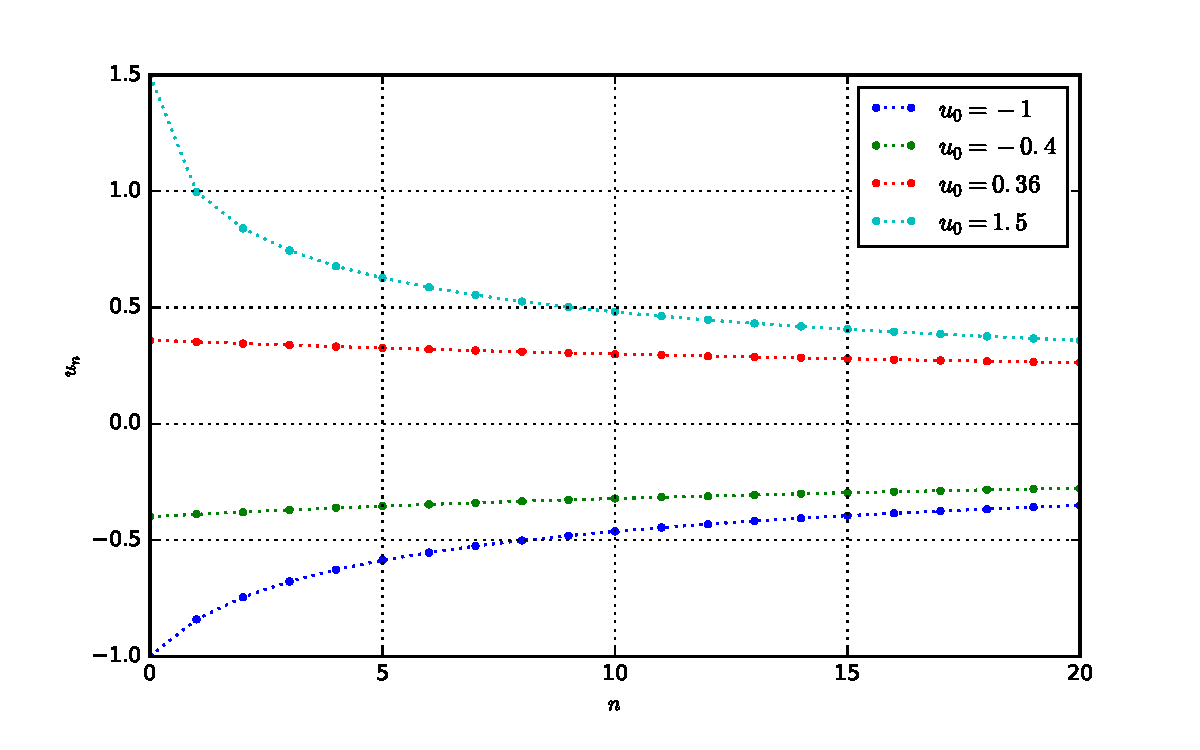
\includegraphics[width=\textwidth]{chope.pdf}
\end{figure}
\end{frame}

\begin{frame}[fragile]
\begin{block}{\textbf{Correction de l'exercice 5}}
\begin{lstlisting}from numpy import sin
def suite(u0, N):
    termes = [u0]
    for i in range(N+1):
        ui = termes[-1]
        termes.append(sin(ui))
    return termes\end{lstlisting}
\end{block}
\end{frame}

\end{document}